\section[O Hardware]{O Hardware}

O hardware Wiring é uma pequena placa de circuito com um microcontrolador atmega644p, construída com base na linguagem Processing. Abaixo algumas características básicas desta placa: 

\begin{alineas}
    \item Pinos digitais de entrada e saída
    \item Pino analógico de entrada
    \item Pino PWM\footnote{\url{https://www.citisystems.com.br/pwm/}} de saída
    \item Porta serial (disponível através do conector USB)
    \item Fonte de alimentação de 7 a 12 Volts
\end{alineas}

Possui aplicações em ensino de eletrônica, ensino de programação de computadores, mídia tangível, arte interativa, etc.

Para mais características consultar o site do fabricante\footnote{\url{http://wiring.org.co/hardware/}}

\begin{figure}[htb]
	\caption{\label{wiringS}Placa Wiring S}
	\begin{center}
	    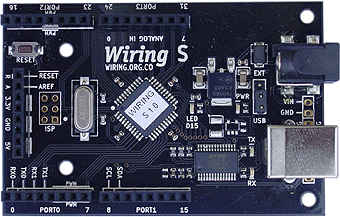
\includegraphics[scale=0.9]{artigo/refs/Rogue_BB_WRS}
	\end{center}
	%\legend{Fonte: Site da 3GPP}
\end{figure}